%%
% This is an Overleaf template for presentations
% using the TUM Corporate Desing https://www.tum.de/cd
%
% For further details on how to use the template, take a look at our
% GitLab repository and browse through our test documents
% https://gitlab.lrz.de/latex4ei/tum-templates.
%
% The tumbeamer class is based on the beamer class.
% If you need further customization please consult the beamer class guide
% https://ctan.org/pkg/beamer.
% Additional class options are passed down to the base class.
%
% If you encounter any bugs or undesired behaviour, please raise an issue
% in our GitLab repository
% https://gitlab.lrz.de/latex4ei/tum-templates/issues
% and provide a description and minimal working example of your problem.
%%

\PassOptionsToClass{onlytextwidth}{beamer}

\documentclass[
  german,            % define the document language (english, german)
  aspectratio=169,    % define the aspect ratio (169, 43)
  % handout=2on1,       % create handout with multiple slides (2on1, 4on1)
  % partpage=false,     % insert page at beginning of parts (true, false)
  % sectionpage=true,   % insert page at beginning of sections (true, false)
]{tumbeamer}


% load additional packages
\usepackage{tikz}
\usepackage{circuitikz}
\usepackage{url}
\usepackage{hyperref}
\usepackage{pgf}
\usepackage{pgfplots}
\usepackage{babel}[ngerman]
\usepackage{csquotes}[autostyle]
\usepackage[useregional]{datetime2}
\usepackage{float}
\usepackage{graphicx}
\usepackage{amsmath}
\usepackage{xcolor}
\usepackage[cache=true]{minted}
\usemintedstyle{borland}
\usepackage{listings}


% tikz
\usetikzlibrary{overlay-beamer-styles}
\usetikzlibrary{arrows,backgrounds,positioning,shapes,,patterns,patterns.meta,matrix,arrows,shapes.geometric}

% requires circuitikz >= 1.1.0
% for distros with older distributions, install TeX Live manually
% instead of using your package manager
% see: https://tug.org/texlive/quickinstall.html
\ctikzset{logic ports=ieee}

% minted
\setminted{
    fontsize=\small, 
    frame=none,
    breaklines=true,
}

% image path
\graphicspath{ {./resources/} }

% beamer
\setbeamercolor{footnote}{fg=black}
\setbeamercolor{footnote mark}{fg=black}

% presentation metadata
\title{Übung 06: Kombinatorische\\Schaltungen}
\subtitle{Einführung in die Rechnerarchitektur}
\author{Niklas Ladurner}

\institute{\theChairName\\\theDepartmentName\\\theUniversityName}
\date{\DTMdisplaydate{2024}{11}{22}{-1}}

\footline{\insertauthor~|~\insertshorttitle~|~\insertshortdate}


% macro to configure the style of the presentation
\TUMbeamersetup{
  title page = TUM tower,         % style of the title page
  part page = TUM toc,            % style of part pages
  section page = TUM toc,         % style of section pages
  content page = TUM more space,  % style of normal content pages
  tower scale = 1.0,              % scaling factor of TUM tower (if used)
  headline = TUM threeliner,      % which variation of headline to use
  footline = TUM default,         % which variation of footline to use
  % configure on which pages headlines and footlines should be printed
  headline on = {title page},
  footline on = {every page, title page=false},
}

\begin{document}

\maketitle

\begin{frame}[c, fragile]{}{}
  \begin{center}
    \LARGE  Keine Garantie für die Richtigkeit der Tutorfolien.

    \Large Bei Unklarheiten/Unstimmigkeiten haben VL/ZÜ-Folien recht!
  \end{center}
\end{frame}

\begin{frame}[c, fragile]{Boolesche Funktionen}{}
  \centering
  \begin{columns}[T]
    \begin{column}{0.3\textwidth}
      \centering
      OR-Gatter

      \vspace{0.2cm}

      \begin{circuitikz}
        \draw (0,0) node[or port] (or) {};
        \draw (or.in 1) node[left] {$A$};
        \draw (or.in 2) node[left] {$B$};
        \draw (or.out) -- ++(0.5,0) node[right] {$A \lor B$};
      \end{circuitikz}

      \vspace{-0.3cm}

      \[
        \begin{array}{|c|c|c|}
          \hline
          A & B & A \lor B \\
          \hline
          0 & 0 & 0        \\
          0 & 1 & 1        \\
          1 & 0 & 1        \\
          1 & 1 & 1        \\
          \hline
        \end{array}
      \]

    \end{column}

    \begin{column}{0.3\textwidth}
      \centering
      AND-Gatter

      \vspace{0.2cm}

      \begin{circuitikz}
        \draw (0,0) node[and port] (and) {};
        \draw (and.in 1) node[left] {$A$};
        \draw (and.in 2) node[left] {$B$};
        \draw (and.out) -- ++(0.5,0) node[right] {$A \land B$};
      \end{circuitikz}

      \vspace{-0.3cm}

      \[
        \begin{array}{|c|c|c|}
          \hline
          A & B & A \land B \\
          \hline
          0 & 0 & 0         \\
          0 & 1 & 0         \\
          1 & 0 & 0         \\
          1 & 1 & 1         \\
          \hline
        \end{array}
      \]

    \end{column}

    \begin{column}{0.3\textwidth}
      \centering
      NOT-Gatter

      \vspace{0.2cm}

      \begin{circuitikz}
        \draw (0,0) node[not port] (not) {};
        \draw (not.in) -- ++(-0.5,0) node[left] {$A$};
        \draw (not.out) -- ++(0.5,0) node[right] {$\lnot A$};
      \end{circuitikz}

      \vspace{-0.3cm}

      \[
        \begin{array}{|c|c|}
          \hline
          A & \lnot A \\
          \hline
          0 & 1       \\
          1 & 0       \\
          \hline
        \end{array}
      \]

    \end{column}

  \end{columns}
\end{frame}

\begin{frame}[c, fragile]{Boolesche Funktionen}{}
  \centering
  \begin{columns}[T]
    \begin{column}{0.5\textwidth}
      \centering
      XOR-Gatter

      \vspace{0.2cm}

      \begin{circuitikz}
        \draw (0,0) node[xor port] (or) {};
        \draw (or.in 1) node[left] {$A$};
        \draw (or.in 2) node[left] {$B$};
        \draw (or.out) -- ++(0.5,0) node[right] {$A \oplus B$};
      \end{circuitikz}

      \vspace{-0.3cm}

      \[
        \begin{array}{|c|c|c|}
          \hline
          A & B & A \oplus B \\
          \hline
          0 & 0 & 0        \\
          0 & 1 & 1        \\
          1 & 0 & 1        \\
          1 & 1 & 0        \\
          \hline
        \end{array}
      \]

    \end{column}

    \begin{column}{0.5\textwidth}
      \centering
      XNOR-Gatter

      \vspace{0.2cm}

      \begin{circuitikz}
        \draw (0,0) node[xnor port] (or) {};
        \draw (or.in 1) node[left] {$A$};
        \draw (or.in 2) node[left] {$B$};
        \draw (or.out) -- ++(0.5,0) node[right] {$A\leftrightarrow B$};
      \end{circuitikz}

      \vspace{-0.3cm}

      \[
        \begin{array}{|c|c|c|}
          \hline
          A & B & A\leftrightarrow B\\
          \hline
          0 & 0 & 1        \\
          0 & 1 & 0        \\
          1 & 0 & 0        \\
          1 & 1 & 1        \\
          \hline
        \end{array}
      \]
    \end{column}


  \end{columns}
\end{frame}

\begin{frame}[c, fragile]{Definitionen}{}
 \begin{block}{Funktionale Vollständigkeit}
      Eine Menge $\mathcal{F}$ boolescher Funktionen heißt funktional vollständig, falls alle booleschen Funktionen als Kombination von $f_i\in\mathcal{F}$ darstellbar sind. Beispiel: $\{\wedge, \neg\}$
 \end{block}
 \vfill
 \begin{block}{Dualität}
  Gegeben eine boolesche Formel $f$, erhält man den dazugehörigen dualen Ausdruck $f^D$ durch Ersetzung: $\{0\mapsto 1; 1\mapsto 0; \wedge\mapsto\vee; \vee\mapsto\wedge\}$. Es gilt $f \Leftrightarrow f^D$.\footnotemark
\end{block}
\footnotetext{Aussage lediglich über Wahrheitsgehalt der Formeln, nicht über Erfüllbarkeitsäquivalenz}
\end{frame}

\begin{frame}[c, fragile]{Gesetze der booleschen Algebra}{}
  \begin{itemize}
    \item Identität: $x+0=x$, $x\cdot 1=x$ \footnote[1]{In ERA werden sowohl die Schreibweisen $\wedge/\vee$ als auch $\cdot / +$ akzeptiert, solange sie einheitlich verwendet werden.}
    \item Idempotenz: $x+x=x$, $x\cdot x=x$
    \item Komplementärgesetz: $x+\overline{x}=1$, $x\cdot\overline{x}=0$
    \item Involution: $\overline{\overline{x}}=x$
    \item De Morgan: $\overline{x+y}=\overline{x}\cdot\overline{y}$ und $\overline{x\cdot y}=\overline{x}+\overline{y}$
    \item Absorption: $x+(x\cdot y)=x$, $x\cdot(x+y)=x$
    \item Distributivität: $x\cdot(y+z)=(x\cdot y)+ (x\cdot z)$ und $x+(y\cdot z)=(x+y)\cdot (x+z)$
  \end{itemize}
\end{frame}

\begin{frame}[c, fragile]{Normalformen}{}
  \begin{columns}[c]
    \begin{column}{0.5\textwidth}
      \begin{itemize}
        \item Konjunktive Normalform (OR in den Klammern, AND dazwischen): $(x+y) \cdot (x+\overline{y})$
        \item Disjunktive Normalform (AND in den Klammern, OR dazwischen): $(x\cdot y) + (x\cdot\overline{y})$
      \end{itemize}
    \end{column}
    \begin{column}{0.5\textwidth}
      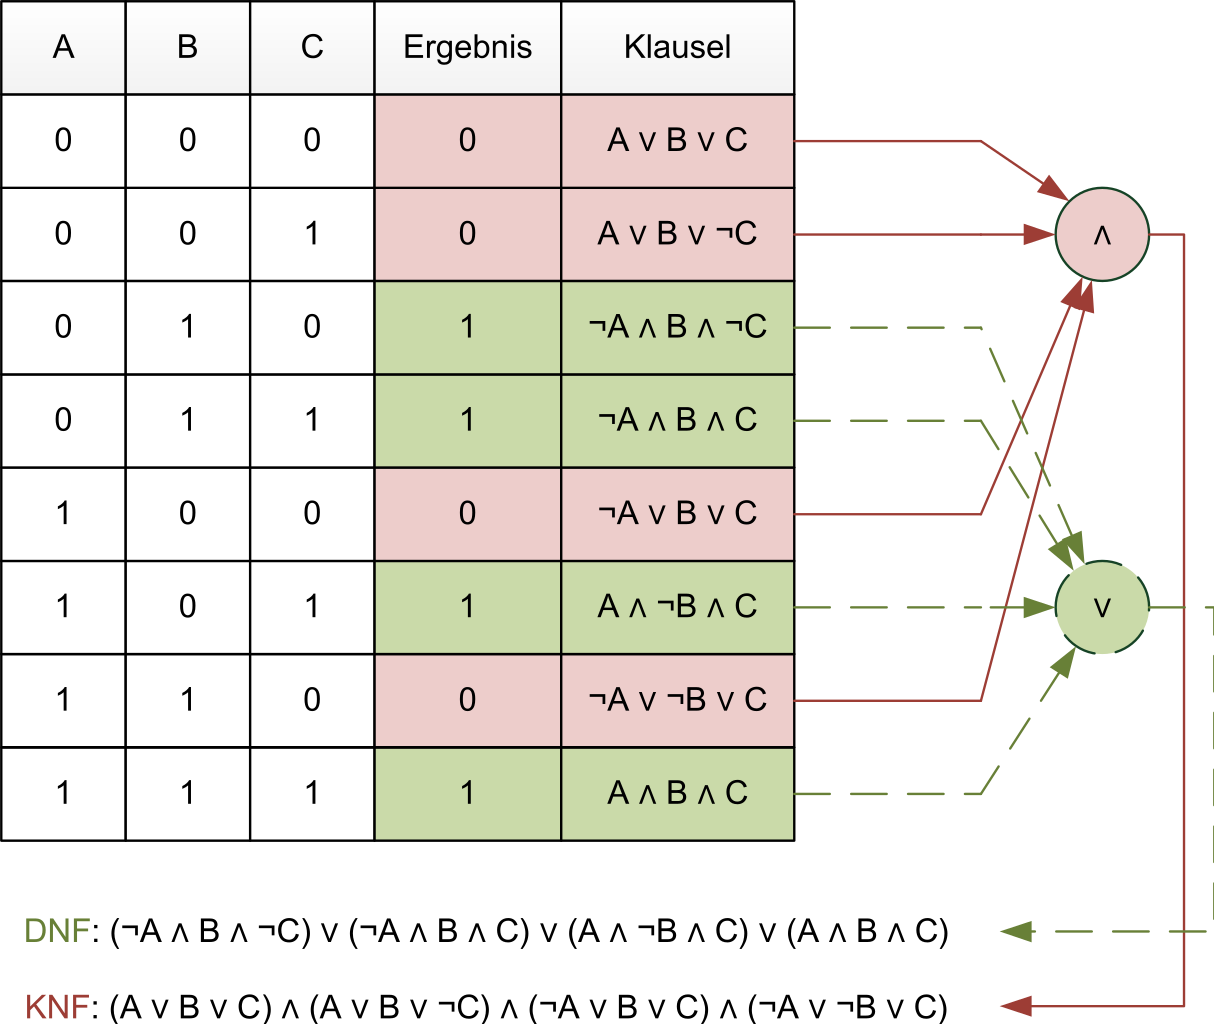
\includegraphics[width=\textwidth]{resources/w06_knf_dnf}
      \centering\scriptsize{Quelle: \href{https://de.wikipedia.org/wiki/Konjunktive_Normalform}{Wikipedia}}
    \end{column}
  \end{columns}
\end{frame}

\begin{frame}[c, fragile]{}{}
  \begin{center}
    \LARGE Fragen?
  \end{center}
\end{frame}

\begin{frame}[c, fragile]{Artemis-Hausaufgaben}{}
  \begin{itemize}
    \item \enquote{H06 --- 16-Segment-Display} bis 01.12.2024 23:59 Uhr
    \item Wahrheitstabellen, Logiksynthese, Implementierung in \href{https://github.com/hneemann/Digital}{Digital}
    \item Vorgehen: \begin{enumerate}
    \item Wahrheitstabelle nach Aufgabenstellung aufstellen
    \item Formeln mittels NAND darstellen
    \item Schaltung zeichnen
    \end{enumerate}
  \end{itemize}
\end{frame}

\begin{frame}[c, fragile]{Links}{}
  \begin{itemize}
    \item Zulip: \href{https://zulip.in.tum.de/#narrow/stream/2661-ERA-Tutorium---Do-1600-1}{\enquote{ERA Tutorium - Do-1600-1}}
          bzw. \href{https://zulip.in.tum.de/#narrow/stream/2675-ERA-Tutorium---Fr-1500-2 }{\enquote{ERA Tutorium - Fr-1500-2}}
    \item \href{https://riscv.org/wp-content/uploads/2017/05/riscv-spec-v2.2.pdf}{RISC-V-Spezifikation}
    \item \href{https://www.moodle.tum.de/course/view.php?id=100633}{ERA-Moodle-Kurs}
    \item \href{https://artemis.in.tum.de/courses/401}{ERA-Artemis-Kurs}
    \item \href{https://www.elektronik-kompendium.de/sites/dig/2609191.htm}{Elektronik-Kompendium zu logischen Grundschaltungen}
    \item \href{https://github.com/hneemann/Digital}{Repository: Digital}
  \end{itemize}
\end{frame}

\maketitle

\end{document}
